\documentclass[a4paper,11pt]{ltjsarticle}

\usepackage{amsmath}
\usepackage{amssymb}
\usepackage{bm}
\usepackage[margin=25mm]{geometry}
\usepackage{tikz}
\usetikzlibrary{arrows.meta,calc,positioning}

\title{透視投影と Projection Matrix の導出}
\author{}
\date{}

\begin{document}
\maketitle

\section{投影の種類}

3次元空間を2次元のスクリーンへ写す方法として、主に次の2種類がある。

\begin{itemize}
  \item \textbf{平行投影}: 投射線が互いに平行。遠近による大きさの変化がない。
  \item \textbf{透視投影}: 投射線が視点に集まる。遠い物体ほど小さく見える。
\end{itemize}

以下では透視投影を扱う。

\begin{figure}[htbp]
  \centering
  \begin{tikzpicture}[>=Latex,scale=0.9]
    % Parallel projection
    \begin{scope}[xshift=-4.2cm]
      \node[font=\bfseries] at (0,2.5) {平行投影};
      \draw[thick] (2,-1.5) -- (2,1.8);
      \node[right] at (2,1.55) {screen};
      \draw[thick] (-1.3,-0.8) rectangle (-0.2,0.4);
      \foreach \y in {-0.6,0,0.6} {
        \draw[->] (-2.3,\y) -- (2,\y);
      }
      \node at (0,-2.0) {投射線は平行};
    \end{scope}

    % Perspective projection
    \begin{scope}[xshift=4.2cm]
      \node[font=\bfseries] at (0,2.5) {透視投影};
      \fill ( -2,0) circle (2pt);
      \node[below] at (-2,0) {視点};
      \draw[thick] (2,-1.5) -- (2,1.8);
      \node[right] at (2,1.55) {screen};
      \draw[thick] (-0.3,-0.8) rectangle (0.8,0.4);
      \draw[->] (-2,0) -- (2,1.1);
      \draw[->] (-2,0) -- (2,-1.1);
      \draw[->] (-2,0) -- (2,0.35);
      \node at (0,-2.0) {投射線が視点へ集まる};
    \end{scope}
  \end{tikzpicture}
  \caption{平行投影と透視投影の違い}
\end{figure}

\section{Viewing Volume}

カメラは原点にあり、$-z$ 方向を向いているとする。

透視投影で画面に表示される範囲は四角錐台（viewing frustum）になる。
カメラからの距離を正の値 $n,f$ で表し、

\begin{align*}
  z &= -n && \text{near plane},\\
  z &= -f && \text{far plane},
\end{align*}

とする。ただし $0<n<f$ である。
near plane より手前、far plane より奥のものは最終的に表示しない。

\begin{figure}[htbp]
  \centering
  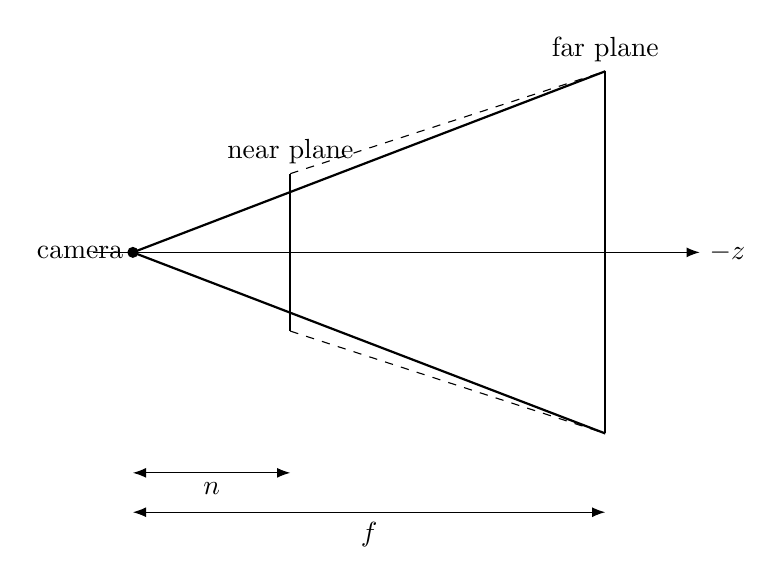
\begin{tikzpicture}[>=Latex,scale=1.0]
    \fill (0,0) circle (2pt);
    \node[left] at (0,0) {camera};
    \draw[->] (-0.5,0) -- (7.2,0) node[right] {$-z$};

    \draw[thick] (2,-1.0) -- (2,1.0);
    \draw[thick] (6,-2.3) -- (6,2.3);
    \node[above] at (2,1.0) {near plane};
    \node[above] at (6,2.3) {far plane};

    \draw[thick] (0,0) -- (6,2.3);
    \draw[thick] (0,0) -- (6,-2.3);
    \draw[dashed] (2,1.0) -- (6,2.3);
    \draw[dashed] (2,-1.0) -- (6,-2.3);

    \draw[<->] (0,-2.8) -- node[below] {$n$} (2,-2.8);
    \draw[<->] (0,-3.3) -- node[below] {$f$} (6,-3.3);
  \end{tikzpicture}
  \caption{透視投影の viewing frustum。可視領域は四角錐台になる。}
\end{figure}

\section{透視投影}

view space 上の点を

\[
  \bm{p}_e = (x_e,y_e,z_e)
\]

とする。near plane 上に投影された座標を $(x',y',-n)$ とすると、相似な三角形から

\begin{align*}
  \frac{x'}{x_e} &= \frac{-n}{z_e},\\
  \frac{y'}{y_e} &= \frac{-n}{z_e}.
\end{align*}

したがって

\begin{align}
  x' &= -n\frac{x_e}{z_e},\\
  y' &= -n\frac{y_e}{z_e}.
\end{align}

$z_e<0$ なので、カメラの前にある点については自然な向きになる。

\begin{figure}[htbp]
  \centering
  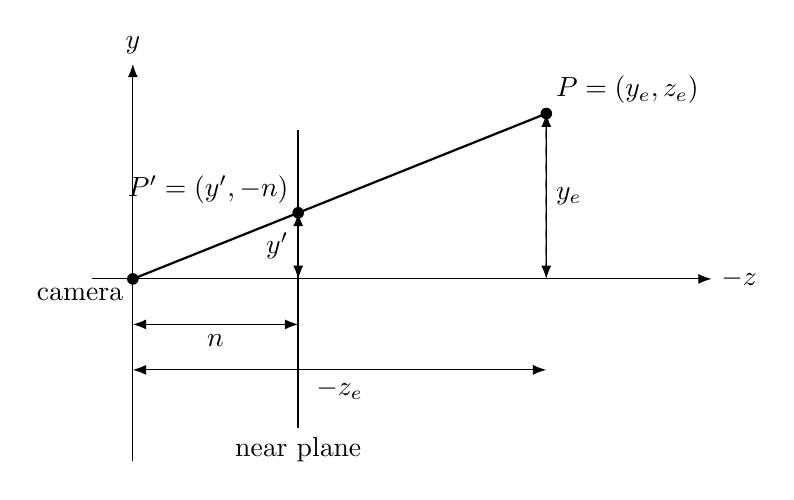
\begin{tikzpicture}[>=Latex,scale=1.05]
    \fill (0,0) circle (2pt);
    \node[below left] at (0,0) {camera};
    \draw[->] (-0.5,0) -- (7,0) node[right] {$-z$};
    \draw[->] (0,-2.2) -- (0,2.6) node[above] {$y$};

    \draw[thick] (2,-1.8) -- (2,1.8);
    \node[below] at (2,-1.8) {near plane};

    \coordinate (P) at (5,2.0);
    \coordinate (Q) at (2,0.8);
    \fill (P) circle (2pt) node[above right] {$P=(y_e,z_e)$};
    \fill (Q) circle (2pt) node[above left] {$P'=(y',-n)$};
    \draw[thick] (0,0) -- (P);

    \draw[dashed] (P) -- (5,0);
    \draw[dashed] (Q) -- (2,0);
    \draw[<->] (0,-0.55) -- node[below] {$n$} (2,-0.55);
    \draw[<->] (0,-1.1) -- node[below] {$-z_e$} (5,-1.1);
    \draw[<->] (5,0) -- node[right] {$y_e$} (P);
    \draw[<->] (2,0) -- node[left] {$y'$} (Q);
  \end{tikzpicture}
  \caption{相似三角形による透視投影。$x$ 方向も全く同じ関係になる。}
\end{figure}

ここで問題になるのは $1/z_e$ であり、そのままでは通常の行列積だけで表現できない。

\section{同次座標と Perspective Divide}

同次座標

\[
  (x,y,z,w)
\]

を使い、Projection Matrix によって

\[
  w_{clip}=-z_e
\]

となるようにする。

行列積の後で

\[
  \bm{p}_{ndc}
  =
  \frac{1}{w_{clip}}
  \begin{pmatrix}
    x_{clip}\\
    y_{clip}\\
    z_{clip}
  \end{pmatrix}
\]

と割れば、透視投影に必要な $1/z_e$ を後段の除算で実現できる。
つまり、相似三角形で現れた負号は $w_{clip}=-z_e$ に吸収されている。

\section{FOV と Aspect Ratio}

near plane の幅を $w$、高さを $h$ とする。
縦方向の視野角を $\mathrm{fov}_y$ とすると、

\[
  \frac{h}{2}
  =
  n\tan\left(\frac{\mathrm{fov}_y}{2}\right).
\]

よって

\[
  h
  =
  2n\tan\left(\frac{\mathrm{fov}_y}{2}\right).
\]

aspect ratio を

\[
  a=\frac{w}{h}
\]

とすれば、

\[
  w=ah.
\]

したがって $x,y$ 方向の projection scale は

\begin{align*}
  \frac{2n}{h}
  &=
  \frac{1}{\tan(\mathrm{fov}_y/2)},\\
  \frac{2n}{w}
  &=
  \frac{1}{a\tan(\mathrm{fov}_y/2)}.
\end{align*}

near plane 上の $[-w/2,w/2]$ と $[-h/2,h/2]$ を、NDC の $[-1,1]$ に対応させる。

\begin{figure}[htbp]
  \centering
  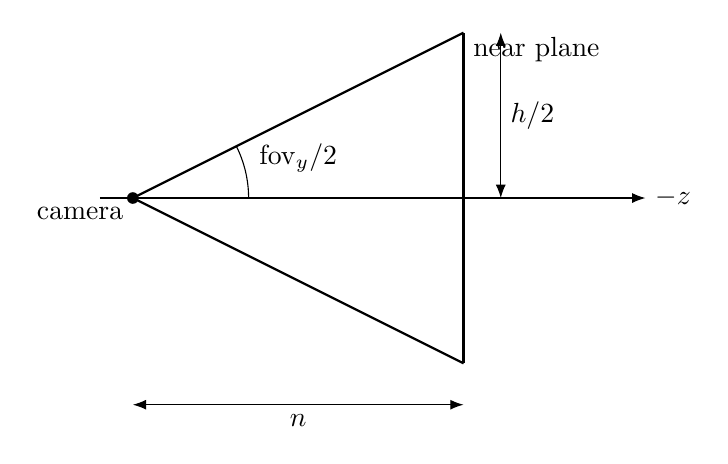
\begin{tikzpicture}[>=Latex,scale=1.05]
    \fill (0,0) circle (2pt);
    \node[below left] at (0,0) {camera};
    \draw[->] (-0.4,0) -- (6.2,0) node[right] {$-z$};
    \draw[thick] (4,-2.0) -- (4,2.0);
    \node[right] at (4,1.8) {near plane};
    \draw[thick] (0,0) -- (4,2.0);
    \draw[thick] (0,0) -- (4,-2.0);

    \draw[<->] (4.45,0) -- node[right] {$h/2$} (4.45,2.0);
    \draw[<->] (0,-2.5) -- node[below] {$n$} (4,-2.5);
    \draw (1.4,0) arc[start angle=0,end angle=26.565,radius=1.4];
    \node at (2.0,0.48) {$\mathrm{fov}_y/2$};
  \end{tikzpicture}
  \caption{$\mathrm{fov}_y$、near 距離 $n$、near plane 高さ $h$ の関係}
\end{figure}

\section{$z$ の正規化}

$x,y$ だけでなく、depth も canonical な範囲へ写す。
OpenGL 型の NDC を使い、

\begin{align*}
  z_e=-n &\quad\longrightarrow\quad z_{ndc}=-1,\\
  z_e=-f &\quad\longrightarrow\quad z_{ndc}=+1
\end{align*}

としたい。

$z$ の clip-space 座標を

\[
  z_{clip}=Az_e+B
\]

と仮定する。$w_{clip}=-z_e$ なので

\[
  z_{ndc}
  =
  \frac{z_{clip}}{w_{clip}}
  =
  \frac{Az_e+B}{-z_e}.
\]

near plane では

\[
  \frac{-An+B}{n}=-1,
\]

したがって

\[
  -An+B=-n.
\]

far plane では

\[
  \frac{-Af+B}{f}=1,
\]

したがって

\[
  -Af+B=f.
\]

この2式を解くと

\begin{align*}
  A &= -\frac{f+n}{f-n},\\
  B &= -\frac{2fn}{f-n}.
\end{align*}

よって

\[
  z_{clip}
  =
  -\frac{f+n}{f-n}z_e
  -\frac{2fn}{f-n}.
\]

perspective divide が入るため、$z_{ndc}$ は view-space の $z$ に対して線形ではない。
depth の分解能はカメラに近い側へ多く割り当てられる。

\section{Projection Matrix}

以上をまとめると、カメラが $-z$ 方向を向く場合の perspective projection matrix は

\[
P=
\begin{pmatrix}
\dfrac{2n}{w} & 0 & 0 & 0 \\
0 & \dfrac{2n}{h} & 0 & 0 \\
0 & 0 & -\dfrac{f+n}{f-n} & -\dfrac{2fn}{f-n} \\
0 & 0 & -1 & 0
\end{pmatrix}.
\]

$\mathrm{fov}_y$ と aspect ratio を直接使えば、

\[
  s=\frac{1}{\tan(\mathrm{fov}_y/2)}
\]

として

\[
P=
\begin{pmatrix}
\dfrac{s}{a} & 0 & 0 & 0 \\
0 & s & 0 & 0 \\
0 & 0 & -\dfrac{f+n}{f-n} & -\dfrac{2fn}{f-n} \\
0 & 0 & -1 & 0
\end{pmatrix}.
\]

\section{描画までの流れ}

頂点 $\bm{p}_{local}$ に対して、

\[
  \bm{p}_{clip}
  =
  PVM\bm{p}_{local}
\]

とする。

その後、perspective divide によって

\[
  \bm{p}_{ndc}
  =
  \frac{\bm{p}_{clip,xyz}}{w_{clip}}
\]

を得る。

最後に viewport transform を行い、NDC の $[-1,1]$ を画面の pixel 座標へ写す。
画面幅を $W$、高さを $H$ とすれば、SDL のように $y$ 軸が下向きの画面では

\begin{align*}
  x_{screen} &= \frac{x_{ndc}+1}{2}W,\\
  y_{screen} &= \frac{1-y_{ndc}}{2}H.
\end{align*}

\begin{figure}[htbp]
  \centering
  \begin{tikzpicture}[>=Latex,scale=0.95]
    \begin{scope}[xshift=-3.6cm]
      \draw[thick] (-1.8,-1.8) rectangle (1.8,1.8);
      \draw[->] (-2.2,0) -- (2.2,0) node[right] {$x_{ndc}$};
      \draw[->] (0,-2.2) -- (0,2.2) node[above] {$y_{ndc}$};
      \node[below left] at (-1.8,-1.8) {$(-1,-1)$};
      \node[above right] at (1.8,1.8) {$(1,1)$};
      \node at (0,-2.7) {NDC};
    \end{scope}

    \draw[->,very thick] (-0.8,0) -- (0.8,0) node[midway,above] {viewport};

    \begin{scope}[xshift=4.0cm]
      \draw[thick] (0,0) rectangle (4.0,2.25);
      \node[above left] at (0,2.25) {$(0,0)$};
      \node[below right] at (4.0,0) {$(W,H)$};
      \draw[->] (0,2.25) -- (1.2,2.25) node[right] {$+x$};
      \draw[->] (0,2.25) -- (0,1.25) node[below] {$+y$};
      \node at (2.0,-0.6) {SDL screen coordinates};
    \end{scope}
  \end{tikzpicture}
  \caption{NDC から画面 pixel 座標への viewport transform}
\end{figure}

したがって現在の変換パイプラインは

\[
  \text{Local}
  \rightarrow
  \text{Model}
  \rightarrow
  \text{View}
  \rightarrow
  \text{Projection}
  \rightarrow
  \text{Perspective Divide}
  \rightarrow
  \text{NDC}
  \rightarrow
  \text{Viewport}
  \rightarrow
  \text{Pixel}
\]

となる。

\section{Triangle Fill と Edge Function}

画面上の三角形を塗りつぶすときは、まず3頂点の $x,y$ から
axis-aligned bounding box (AABB) を求め、その矩形内の pixel だけを走査する。
三角形の頂点を $A,B,C$ とし、各辺を

\[
  A\rightarrow B,\qquad
  B\rightarrow C,\qquad
  C\rightarrow A
\]

とする。
任意の画面上の点 $P$ が各辺のどちら側にあるかは、2次元外積

\[
  \operatorname{cross}\bigl((u_x,u_y),(v_x,v_y)\bigr)
  =u_xv_y-u_yv_x
\]

の符号で判定できる。

例えば辺 $A\rightarrow B$ に対しては

\[
  E_{AB}(P)
  =
  (B-A)\times(P-A)
\]

を計算する。
三角形の3辺について求めた edge function の符号がすべて同じなら、
$P$ は三角形内部にある。
画面座標では viewport transform により $y$ 軸が反転しているため、
実装では winding に依存せず

\[
  (E_0\ge0\land E_1\ge0\land E_2\ge0)
  \quad\text{or}\quad
  (E_0\le0\land E_1\le0\land E_2\le0)
\]

のように判定してもよい。

\subsection{Pixel center sampling と $+0.5$}

framebuffer 上の整数 index $(x,y)$ は1 pixel の領域を表す。
例えば pixel $(10,20)$ は概念的には

\[
  10\le x<11,\qquad 20\le y<21
\]

の領域を占める。
その中心は

\[
  (10.5,20.5)
\]

なので、三角形内判定では一般に

\[
  P=(x+0.5,\ y+0.5)
\]

をサンプル点として使う。
一方、実際に framebuffer へ書き込む index はそのまま

\[
  \texttt{index}=yW+x
\]

でよい。
$+0.5$ は配列 index をずらすためではなく、pixel のどの位置を代表点として
coverage 判定するかを決めるためのものである。

\subsection{Edge Function の逐次更新}

各 pixel ごとに外積を最初から計算すると、内側ループで多数の乗算と減算が必要になる。
しかし edge function は $x,y$ の一次式なので、隣の pixel の値は定数加算だけで求められる。

辺ベクトルを

\[
  \bm{e}=B-A=(d_x,d_y)
\]

とする。現在使っている edge function を

\[
  E(x,y)
  =
  (B-A)\times(P-A)
\]

とすると、$P=(x,y)$ に対して

\begin{align*}
  E(x,y)
  &=d_x(y-a_y)-d_y(x-a_x)\\
  &=-d_yx+d_xy+\text{constant}
\end{align*}

と書ける。
したがって右隣の pixel では

\[
  E(x+1,y)=E(x,y)-d_y,
\]

1行下では

\[
  E(x,y+1)=E(x,y)+d_x
\]

となる。
つまり最初の1 pixel だけ通常の外積を計算すれば、その後は

\begin{align*}
  \text{right step} &: \quad E\leftarrow E-d_y,\\
  \text{down step}  &: \quad E_{\mathrm{row}}\leftarrow E_{\mathrm{row}}+d_x
\end{align*}

だけで走査できる。

実装上は、各行の左端の値と、その行を横に走査する作業用の値を分けて持つ。

\begin{verbatim}
row_e0 = Edge(A, B, first_pixel)
row_e1 = Edge(B, C, first_pixel)
row_e2 = Edge(C, A, first_pixel)

for y = min_y ... max_y:
    e0 = row_e0
    e1 = row_e1
    e2 = row_e2

    for x = min_x ... max_x:
        if signs of e0,e1,e2 match:
            draw pixel

        e0 -= (B-A).y
        e1 -= (C-B).y
        e2 -= (A-C).y

    row_e0 += (B-A).x
    row_e1 += (C-B).x
    row_e2 += (A-C).x
\end{verbatim}

この方法でも調べる pixel 数自体は AABB の面積に比例するため、計算量の次数は変わらない。
ただし各 pixel で外積を再計算する必要がなくなり、inner loop をほぼ比較と加算だけにできる。
同じ edge function は後で barycentric coordinate や depth interpolation を求める際にも再利用できる。

\section{Barycentric Coordinate（重心座標）}

三角形 $ABC$ の内部だけに特別な式を作るのではなく、まず三角形そのものを
1つの affine なローカル座標系として考える。
頂点 $A$ を基準点とし、2本の辺

\[
  B-A,\qquad C-A
\]

を基底方向として、平面上の点 $P$ を

\begin{equation}
  P=A+s(B-A)+t(C-A)
\end{equation}

と表す。
$B-A$ と $C-A$ が平行でなければ、$s,t\in\mathbb{R}$ とすることで
この式は三角形内部だけでなく平面全体を表せる。

展開すると

\begin{align*}
  P
  &=A+sB-sA+tC-tA\\
  &=(1-s-t)A+sB+tC.
\end{align*}

ここで

\[
  \alpha=1-s-t,\qquad
  \beta=s,\qquad
  \gamma=t
\]

と置けば

\begin{equation}
  \boxed{
    P=\alpha A+\beta B+\gamma C,
    \qquad
    \alpha+\beta+\gamma=1
  }
\end{equation}

となる。この $(\alpha,\beta,\gamma)$ が三角形 $ABC$ に対する
barycentric coordinate である。

\subsection{$\alpha+\beta+\gamma=1$ の意味}

重みの和が1という条件は、単に「三角形を3つに分割した面積の合計が1になる」から
後付けした条件ではない。
もともとの affine 座標

\[
  P=A+s(B-A)+t(C-A)
\]

を書き換えた時点で必然的に現れる。

また、この条件によって座標表現が原点の選び方に依存しなくなる。
すべての点を同じベクトル $d$ だけ平行移動して

\[
  A'=A+d,\quad B'=B+d,\quad C'=C+d
\]

とすると

\begin{align*}
  \alpha A'+\beta B'+\gamma C'
  &=\alpha A+\beta B+\gamma C
    +(\alpha+\beta+\gamma)d\\
  &=P+d
\end{align*}

となる。最後の等号が成り立つのは
$\alpha+\beta+\gamma=1$ だからである。
したがって barycentric coordinate は通常の線形座標というより、
平行移動を含む affine geometry に自然な座標になっている。

\subsection{三角形内部と外部}

barycentric coordinate 自体は三角形の外でも定義できる。
三角形内部にある条件は

\begin{equation}
  \boxed{
    \alpha\ge0,\qquad
    \beta\ge0,\qquad
    \gamma\ge0,
    \qquad
    \alpha+\beta+\gamma=1
  }
\end{equation}

である。
このように、係数の和が1で、さらにすべての係数が非負である線形結合を
\textbf{convex combination（凸結合）}という。

一方、点 $P$ が三角形の外へ出ると、和は1のままだが少なくとも1つの係数が負になる。
したがって barycentric coordinate は座標表現と point-in-triangle 判定を
同じ式で扱える。

\subsection{外積による係数の導出}

式

\[
  P-A=\beta(B-A)+\gamma(C-A)
\]

から $\beta,\gamma$ を直接求める。
記号を簡単にするため

\[
  u=B-A,\qquad
  v=C-A,\qquad
  q=P-A
\]

と置くと

\[
  q=\beta u+\gamma v
\]

である。

両辺と $v$ の外積を取ると

\begin{align*}
  q\times v
  &=(\beta u+\gamma v)\times v\\
  &=\beta(u\times v)+\gamma(v\times v)\\
  &=\beta(u\times v),
\end{align*}

なので

\begin{equation}
  \boxed{
    \beta=
    \frac{(P-A)\times(C-A)}
         {(B-A)\times(C-A)}
  }
\end{equation}

となる。

同様に $u$ と外積を取れば

\begin{equation}
  \boxed{
    \gamma=
    \frac{(B-A)\times(P-A)}
         {(B-A)\times(C-A)}
  }
\end{equation}

を得る。最後に

\[
  \alpha=1-\beta-\gamma
\]

とすればよい。

2次元外積の絶対値は2つのベクトルが張る平行四辺形の面積なので、
$\frac12$ を掛ければ三角形の面積になる。
分子と分母の両方に同じ $\frac12$ が現れて打ち消し合うため、上の式は
そのまま面積比として解釈できる。

\begin{align*}
  \alpha&=\frac{\operatorname{area}(PBC)}{\operatorname{area}(ABC)},\\
  \beta &=\frac{\operatorname{area}(PCA)}{\operatorname{area}(ABC)},\\
  \gamma&=\frac{\operatorname{area}(PAB)}{\operatorname{area}(ABC)}.
\end{align*}

したがって、例えば $P$ が $A$ に近づくほど
$\operatorname{area}(PBC)$ は元の三角形 $ABC$ の面積に近づき、
$\alpha\rightarrow1$ となる。

\subsection{Edge Function との対応}

前節で使った edge function を

\begin{align*}
  E_{AB}(P)&=(B-A)\times(P-A),\\
  E_{BC}(P)&=(C-B)\times(P-B),\\
  E_{CA}(P)&=(A-C)\times(P-C)
\end{align*}

とする。
三角形全体の符号付き2倍面積を

\[
  S=(B-A)\times(C-A)
\]

とすれば、winding が一致している場合

\begin{equation}
  \boxed{
    \alpha=\frac{E_{BC}(P)}{S},\qquad
    \beta =\frac{E_{CA}(P)}{S},\qquad
    \gamma=\frac{E_{AB}(P)}{S}
  }
\end{equation}

となる。

つまり rasterizer が三角形内部判定のためにすでに計算している3つの edge value は、
そのまま barycentric weight の分子として再利用できる。
例えば $E_{AB}$ は辺 $AB$ から点 $P$ までの符号付き面積を表し、
$P=C$ なら三角形全体の面積 $S$ になるため $\gamma=1$、
$P$ が辺 $AB$ 上なら $E_{AB}=0$ なので $\gamma=0$ になる。

\subsection{Barycentric Interpolation と Depth Buffer}

三角形の各頂点に値

\[
  f_A,\qquad f_B,\qquad f_C
\]

が与えられており、その値が三角形上で affine に変化するとき、点 $P$ の値は

\begin{equation}
  \boxed{
    f(P)=\alpha f_A+\beta f_B+\gamma f_C
  }
\end{equation}

で求められる。

depth buffer では、Projection と perspective divide 後の各頂点の
$z_{ndc}$ を保持しておき、screen-space の barycentric weight を使って

\begin{equation}
  z_P
  =\alpha z_{A,ndc}
  +\beta z_{B,ndc}
  +\gamma z_{C,ndc}
\end{equation}

と補間する。
現在の OpenGL 型 NDC では

\[
  \text{near}\rightarrow-1,
  \qquad
  \text{far}\rightarrow+1
\]

なので、小さい depth ほどカメラに近い。
したがって pixel index $i$ に対して

\begin{verbatim}
if depth < z_buffer[i]:
    z_buffer[i] = depth
    frame_buffer[i] = color
\end{verbatim}

とすれば、最も手前の fragment だけを残せる。
$z$ buffer は毎 frame、例えば $+\infty$ へ clear しておく。

ここで補間するのは view-space の $z$ ではなく、perspective divide 後の
$z_{ndc}$ であることに注意する。
view-space の $z$ は透視投影後の screen space に対して線形ではない。

一方、texture UV、view/world position、normal などの属性は、単純な screen-space
barycentric interpolation だけでは透視投影と整合しない。
これらには後で $1/w$ を使う perspective-correct interpolation が必要になる。

\subsection{一般化: Simplex と凸性}

barycentric coordinate は三角形だけの概念ではない。
$d$ 次元では $d+1$ 個の affinely independent な点が作る
\textbf{simplex} に対して同じ考え方を使える。

\begin{center}
\begin{tabular}{c|c|c}
次元 & 頂点数 & simplex \\
\hline
1 & 2 & 線分 \\
2 & 3 & 三角形 \\
3 & 4 & 四面体
\end{tabular}
\end{center}

例えば3次元の四面体では

\[
  P=\alpha A+\beta B+\gamma C+\delta D,
  \qquad
  \alpha+\beta+\gamma+\delta=1
\]

となり、4係数は一意に定まる。

一方、2次元で4頂点を使うと未知係数が4つあるのに対し、
$x,y$ と係数和の条件を合わせても式は3本しかないため、一般には重みは一意に定まらない。
このため任意の四角形を1組の単純な barycentric weight だけで扱うことはできず、
CG では三角形へ分割して各三角形ごとに barycentric coordinate を使う方法が自然になる。

また、係数の和が1で全係数が非負な点全体は頂点集合の
\textbf{convex hull（凸包）}になる。
三角形は2次元の simplex であり、それ自身が凸なので、
barycentric coordinate、inside 判定、補間、凸性がすべて同じ数学の上でつながっている。

\end{document}
